\documentclass[11pt,a4paper]{article}
\usepackage[utf8]{inputenc}
\usepackage{amsmath,amsfonts,amssymb}
\usepackage{graphicx}
\usepackage{geometry}
\geometry{margin=1in}
\usepackage{booktabs}
\usepackage{hyperref}
\usepackage{float}
\usepackage{xcolor}
\usepackage{array}

\definecolor{darkbg}{HTML}{0d121f}
\definecolor{lighttext}{HTML}{e2e8f0}
\definecolor{primary}{HTML}{8b5cf6}
\definecolor{secondary}{HTML}{0dd5c5}
\definecolor{accent}{HTML}{10b981}

\pagecolor{darkbg}
\color{lighttext}

\hypersetup{
    colorlinks=true,
    linkcolor=secondary,
    urlcolor=secondary,
    citecolor=accent
}

\title{\textbf{EE3621: Digital Signal Processing} \\ \Large Lecture 28: From Adaptive Filtering to Machine Learning --- The DSP $\leftrightarrow$ ML Dictionary \\ \large (III B.Tech EEE)}
\author{Comprehensive Lecture Notes \& Faculty Textbook Reference}
\date{}

\begin{document}

\maketitle

\noindent\rule{\textwidth}{0.5pt}

\section*{Lecture Plan \& Objectives (40 Minutes Breakdown)}
\begin{itemize}
    \item \textbf{00:00 -- 06:00:} FIR $\to$ single-layer ANN / convolution layer; LMS $=$ stochastic gradient descent (ADALINE).
    \item \textbf{06:00 -- 13:00:} IIR $\to$ RNN: poles as eigenvalues, vanishing/exploding gradients, gated units, state-space models; EMA momentum as an IIR lowpass.
    \item \textbf{13:00 -- 20:00:} Fourier transform $\leftrightarrow$ eigenvectors: complex exponentials, circulant matrices, PCA/KLT, eigenvalue spread in LMS; noise filtering by SVD.
    \item \textbf{20:00 -- 30:00:} Non-local means $\to$ BM3D $\to$ Transformers (attention); positional encoding as phasors of geometrically spaced frequencies.
    \item \textbf{30:00 -- 37:00:} Further analogies (Wiener/regression, Kalman, matched filter, pooling/aliasing, filter banks, residuals, normalization, linear prediction).
    \item \textbf{37:00 -- 40:00:} Worked numerical examples, honest limits of each analogy, exam traps.
\end{itemize}

\noindent\rule{\textwidth}{0.5pt}

\section{1. LEARNING OBJECTIVES}
Students will be able to:
\begin{enumerate}
    \item Map the LMS adaptive FIR filter onto a one-neuron network trained with SGD.
    \item Explain why a recurrent layer is a nonlinear IIR filter and relate poles to gradient stability.
    \item State why Fourier bases are the eigenvectors of LTI systems and how PCA/KLT generalizes them.
    \item Apply truncated-SVD denoising and justify it with the Eckart--Young theorem.
    \item Show that non-local-means/BM3D-style patch aggregation is a form of attention.
    \item Show that sinusoidal positional encoding is a bank of phasors, and that a position shift is a phase rotation.
    \item State where each analogy \emph{breaks down}.
\end{enumerate}

\noindent\rule{\textwidth}{0.5pt}

\section{2. THE MASTER DICTIONARY}
\begin{table}[H]
\centering
\small
\begin{tabular}{p{4.0cm}p{4.0cm}p{6.5cm}}
\toprule
\textbf{DSP / Adaptive filtering} & \textbf{Machine learning} & \textbf{Where the link is exact} \\
\midrule
FIR filter $y=\mathbf{w}^T\mathbf{x}$ & Linear neuron / dense layer; 1-D conv layer & Same equation; a conv layer is a bank of FIR filters with shared taps \\
LMS (Widrow--Hoff) & SGD on squared loss; delta rule; ADALINE & Identical update $\mathbf{w}\!\leftarrow\!\mathbf{w}+\mu e\mathbf{x}$ \\
IIR filter & Recurrent network (RNN, LSTM, SSM) & A linear RNN \emph{is} an IIR filter \\
Poles inside unit circle & Spectral radius of $\mathbf{W}_h<1$ & Stability $\leftrightarrow$ vanishing/exploding gradients \\
Fourier basis & Eigenvectors of $\mathbf{R}$, PCA & Complex exponentials diagonalize circulant matrices \\
SVD/subspace denoising & PCA, low-rank approximation, LoRA & Eckart--Young optimality \\
BM3D / non-local means & Self-attention, Vision Transformers & NLM weights are Gaussian-kernel softmax attention \\
Sinusoidal positional encoding & Phasors at frequencies $10000^{-2i/d}$ & Shift $\Rightarrow$ rotation (shift theorem) \\
Wiener filter, $\mathbf{R}\mathbf{w}=\mathbf{p}$ & Linear regression normal equations & Same equations \\
Exponential average & Momentum / Adam moments & First-order IIR lowpass \\
\bottomrule
\end{tabular}
\end{table}

\noindent\rule{\textwidth}{0.5pt}

\section{3. FIR FILTER $\to$ ANN; LMS $\to$ GRADIENT DESCENT}

\subsection{3.1 Same equation}
FIR / adaptive transversal filter and a single neuron before the activation:
\begin{equation}
y[n] = \sum_{k=0}^{M-1} w_k\,x[n-k] = \mathbf{w}^T\mathbf{x}[n] \qquad\longleftrightarrow\qquad z = \mathbf{w}^T\mathbf{x} + b,\quad a = \varphi(z).
\end{equation}
The tapped delay line supplies $\mathbf{x}[n]$; in ML the inputs are arbitrary features. Adding a nonlinearity $\varphi$ gives a perceptron; stacking layers gives a multilayer perceptron (MLP).

\subsection{3.2 Convolutional layers}
A 1-D convolutional layer slides the \emph{same} FIR filter over the signal (weight sharing = time invariance), uses several filters (channels $=$ a filter bank), applies a nonlinearity, then downsamples. Image CNNs are 2-D FIR filters. Most deep-learning libraries compute cross-correlation, not flipped-kernel convolution, but the difference is only a flip of $\mathbf{w}$.

\subsection{3.3 LMS $=$ SGD}
With squared loss $\ell = \tfrac12 e^2$, $e = d - \mathbf{w}^T\mathbf{x}$, one SGD step is
\begin{equation}
\mathbf{w}\leftarrow \mathbf{w} - \mu\nabla_{\mathbf{w}}\ell = \mathbf{w} + \mu\, e\,\mathbf{x}.
\end{equation}
This is the LMS update of Lecture 27. Backpropagation is the same rule with the chain rule applied through layers: $\delta_{\text{layer}}$ plays the role of $e$.
\begin{itemize}
    \item \textbf{Step size:} $\mu$ is the learning rate; the bound $0<\mu<2/\lambda_{\max}(\mathbf{R})$ is the quadratic-loss stability limit for gradient descent.
    \item \textbf{Misadjustment vs.\ speed:} large $\mu$ = fast but noisy; the LMS trade-off is the learning-rate/mini-batch trade-off.
    \item \textbf{Convergence modes:} the error along eigenvector $\mathbf{q}_i$ of $\mathbf{R}$ decays as $(1-\mu\lambda_i)^n$. Large \emph{eigenvalue spread} $\lambda_{\max}/\lambda_{\min}$ gives slow convergence --- the reason for input whitening/normalization in ML and for RLS/Adam-type preconditioning.
    \item \textbf{Regularization:} leaky LMS ($\mathbf{w}\leftarrow(1-\mu\gamma)\mathbf{w}+\dots$) $=$ weight decay / ridge; diagonal loading of $\mathbf{R}$ $=$ ridge regression.
    \item \textbf{Normalized LMS} $\mu/(\epsilon+\|\mathbf{x}\|^2)$ $\leftrightarrow$ normalized/adaptive learning rates.
    \item \textbf{RLS} $\leftrightarrow$ Newton/second-order methods.
\end{itemize}

\subsection{3.4 Wiener filter $=$ linear regression}
The Wiener equations $\mathbf{R}\mathbf{w}^\ast=\mathbf{p}$ are the normal equations $\mathbf{X}^T\mathbf{X}\mathbf{w}=\mathbf{X}^T\mathbf{d}$ of least squares, with sample averages replacing expectations. Adaptive filtering is online learning; Wiener is the batch solution.

\noindent\rule{\textwidth}{0.5pt}

\section{4. IIR FILTER $\to$ RECURRENT NEURAL NETWORK}

\subsection{4.1 Feedback gives memory}
\begin{equation}
\text{IIR: } y[n] = \sum_{k} b_k x[n-k] - \sum_{k\ge1} a_k y[n-k] \qquad
\text{RNN: } \mathbf{h}_t = \varphi(\mathbf{W}_h\mathbf{h}_{t-1} + \mathbf{W}_x\mathbf{x}_t + \mathbf{b}).
\end{equation}
Remove the nonlinearity ($\varphi=\text{identity}$): $\mathbf{h}_t = \mathbf{W}_h\mathbf{h}_{t-1} + \mathbf{W}_x\mathbf{x}_t$, a state-space IIR filter with
\begin{equation}
\mathbf{H}(z) = (\mathbf{I}-\mathbf{W}_h z^{-1})^{-1}\mathbf{W}_x, \qquad \text{poles} = \text{eigenvalues of } \mathbf{W}_h.
\end{equation}
\begin{itemize}
    \item \textbf{Stability:} BIBO stable iff all eigenvalues of $\mathbf{W}_h$ lie inside the unit circle.
    \item \textbf{Vanishing/exploding gradients:} backprop through time multiplies by $\mathbf{W}_h^T$ repeatedly; the gradient after $k$ steps scales like $\rho(\mathbf{W}_h)^k$. Poles inside $\to$ vanish (short memory); outside $\to$ explode; near $|z|=1$ $\to$ long memory. This is the impulse response $a^n u[n]$ of a one-pole filter.
    \item \textbf{Nonlinear case:} $\tanh$ bounds the state, which prevents blow-up of the forward pass but not of the gradients.
\end{itemize}

\subsection{4.2 Gated RNNs as adaptive-pole IIR filters}
A one-pole IIR $y[n] = a\,y[n-1] + (1-a)x[n]$ has fixed leakage $a$. An LSTM/GRU cell state $c_t = f_t\odot c_{t-1} + i_t\odot g_t$ is the same recursion with a \emph{signal-dependent pole} $f_t\in(0,1)$ (forget gate) and input gain $i_t$. Modern \textbf{state-space models} (S4, Mamba) are explicitly discretized linear systems (zero-order hold/bilinear transform, exactly Lectures 15--27) computed by convolution or recurrence.

\subsection{4.3 Worked Example 28.1: EMA momentum is an IIR lowpass}
Gradient momentum / exponential moving average: $m_t = \beta m_{t-1} + (1-\beta) g_t$. So $H(z) = \frac{1-\beta}{1-\beta z^{-1}}$ with a single pole at $z=\beta$.
\begin{itemize}
    \item DC gain: $H(1) = 1$. Gain at $\omega=\pi$: $H(-1) = \frac{1-\beta}{1+\beta}$. For $\beta=0.9$: $0.1/1.9 \approx 0.053$ ($-25.6$\,dB).
    \item Memory: time constant $\tau \approx 1/(1-\beta) = 10$ samples; $-3$\,dB frequency $\omega_c \approx 1-\beta=0.1$\,rad (for $\beta$ near 1).
    \item Interpretation: momentum is a lowpass filter on the noisy gradient sequence, suppressing high-frequency gradient noise (just like smoothing in DSP).
\end{itemize}

\noindent\rule{\textwidth}{0.5pt}

\section{5. FOURIER TRANSFORM $\leftrightarrow$ EIGENVECTORS}

\subsection{5.1 Complex exponentials are eigenfunctions of LTI systems}
For input $x[n] = e^{j\omega n}$ and impulse response $h[n]$:
\begin{equation}
y[n] = \sum_k h[k]e^{j\omega(n-k)} = H(e^{j\omega})\,e^{j\omega n}.
\end{equation}
So $e^{j\omega n}$ is an \textbf{eigenvector} and $H(e^{j\omega})$ the \textbf{eigenvalue}. For finite-length periodic (circular) convolution the operator is a \textbf{circulant matrix} $\mathbf{C}$, and
\begin{equation}
\mathbf{C} = \mathbf{F}^{H}\,\mathrm{diag}\big(H[0],\dots,H[N-1]\big)\,\mathbf{F},
\end{equation}
with $\mathbf{F}$ the DFT matrix: the DFT diagonalizes every circulant matrix. This is why convolution becomes multiplication in the frequency domain.

\subsection{5.2 PCA / KLT: data-dependent Fourier}
For a zero-mean random vector with covariance $\mathbf{R}=\mathbf{Q}\boldsymbol{\Lambda}\mathbf{Q}^T$, the Karhunen--Lo\`eve transform uses eigenvectors $\mathbf{Q}$ as an optimal decorrelating basis (this is PCA). For a wide-sense stationary signal, $\mathbf{R}$ is Toeplitz and, as the length grows, asymptotically circulant, so the eigenvectors tend to \textbf{Fourier vectors} and the eigenvalues to the \textbf{power spectral density}:
\begin{equation}
\lambda_i \to S_x(\omega_i).
\end{equation}
Thus the DFT is the KLT of stationary signals, and PCA is the generalization to non-stationary data.

\subsection{5.3 Consequences for adaptive filtering}
$\lambda_{\max}/\lambda_{\min}\to S_{\max}/S_{\min}$: a \emph{coloured} input (large spectral dynamic range) slows LMS; white input gives the fastest, equal-rate convergence. Pre-whitening, transform-domain LMS (DFT/DCT-LMS) and feature normalization in ML are all the same fix.

\subsection{5.4 Other Fourier $\leftrightarrow$ ML links}
FFT-based fast convolution; spectrogram/mel inputs to speech models; Fourier features for coordinate networks ($\sin/\cos$ of random frequencies); Fourier Neural Operators; FNet (token mixing by FFT).

\noindent\rule{\textwidth}{0.5pt}

\section{6. NOISE FILTERING VIA SVD}

\subsection{6.1 Theory}
Any matrix $\mathbf{A}=\mathbf{U}\boldsymbol{\Sigma}\mathbf{V}^T=\sum_i\sigma_i\mathbf{u}_i\mathbf{v}_i^T$. The \textbf{Eckart--Young theorem}: the best rank-$k$ approximation in Frobenius (and spectral) norm is the truncated sum $\mathbf{A}_k=\sum_{i\le k}\sigma_i\mathbf{u}_i\mathbf{v}_i^T$.

Signal $+$ white noise: $\mathbf{Y}=\mathbf{S}+\mathbf{N}$ with $\mathbf{S}$ low rank. Noise spreads \emph{evenly} over all singular values (a noise floor $\approx\sigma_n(\sqrt{m}+\sqrt{n})$), while signal energy concentrates in a few large $\sigma_i$. Keeping only the large ones removes most noise --- a lowpass filter in the \emph{singular spectrum} instead of the frequency spectrum.

\subsection{6.2 DSP usage}
Take a Hankel/Toeplitz matrix of a 1-D signal (a sum of $r$ sinusoids/damped exponentials gives rank $2r$, or $r$ for complex exponentials); truncating its SVD and anti-diagonal averaging is \textbf{Cadzow denoising}. Also: subspace methods (MUSIC, ESPRIT), PCA denoising, singular value thresholding, low-rank adaptation (LoRA) of neural weights.

\subsection{6.3 Worked Example 28.2}
Noisy observation $\mathbf{Y}=\begin{bmatrix}3.1&2.9\\2.9&3.1\end{bmatrix}$. Eigenvalues of this symmetric matrix: $3.1\pm2.9 = 6.0,\;0.2$ with eigenvectors $\frac1{\sqrt2}[1,1]^T$ and $\frac1{\sqrt2}[1,-1]^T$. Singular values: $\sigma_1=6.0$, $\sigma_2=0.2$. Rank-1 truncation:
\begin{equation}
\mathbf{Y}_1 = 6.0\cdot\tfrac12\begin{bmatrix}1&1\\1&1\end{bmatrix}=\begin{bmatrix}3&3\\3&3\end{bmatrix}.
\end{equation}
The rank-one structure (identical rows/columns) is recovered, and the small singular value $0.2$ (the noise-like component) is discarded.

\begin{figure}[H]
\centering
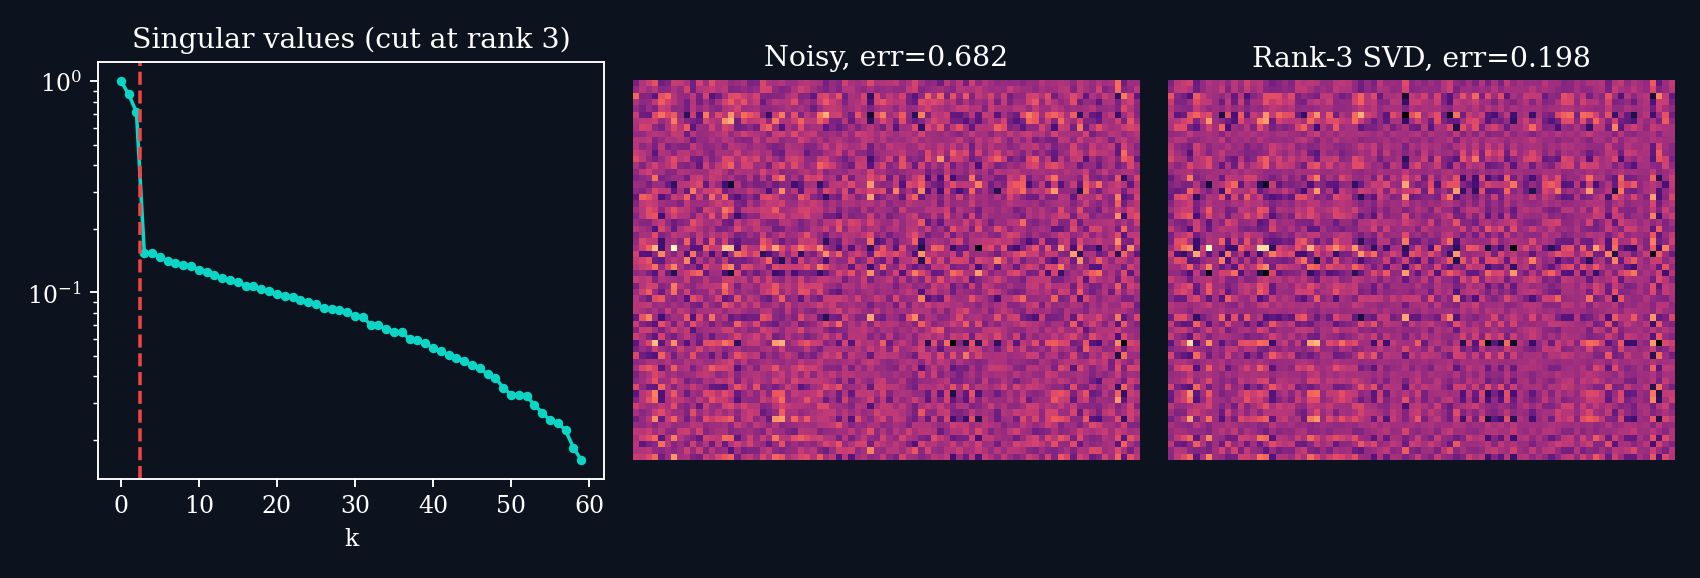
\includegraphics[width=0.95\textwidth]{images/l28_svd_denoise.png}
\caption{Rank-3 matrix plus white noise: the singular-value spectrum shows a sharp drop after 3; truncation reduces the Frobenius error to the true matrix (error values printed in the panels).}
\end{figure}

\noindent\rule{\textwidth}{0.5pt}

\section{7. BM3D $\to$ TRANSFORMERS: NON-LOCAL AGGREGATION}

\subsection{7.1 Non-local means (NLM)}
Pixel/sample $i$ is estimated as a weighted average of \emph{all} samples whose surrounding patches look similar:
\begin{equation}
\hat{x}_i=\sum_j w_{ij}\,x_j,\qquad w_{ij}=\frac{\exp\!\big(-\|\mathbf{p}_i-\mathbf{p}_j\|^2/h^2\big)}{\sum_{j'}\exp\!\big(-\|\mathbf{p}_i-\mathbf{p}_{j'}\|^2/h^2\big)}.
\end{equation}
Compare with scaled dot-product attention
\begin{equation}
\mathrm{Attn}(\mathbf{q}_i)=\sum_j\mathrm{softmax}_j\!\Big(\frac{\mathbf{q}_i^T\mathbf{k}_j}{\sqrt{d}}\Big)\mathbf{v}_j.
\end{equation}
Since $-\|\mathbf{q}-\mathbf{k}\|^2 = 2\mathbf{q}^T\mathbf{k}-\|\mathbf{q}\|^2-\|\mathbf{k}\|^2$ and the $\|\mathbf{q}\|^2$ term cancels inside the softmax, Gaussian-kernel NLM equals dot-product attention when key norms are constant (or are absorbed in a bias). So: \emph{patch} $=$ query/key, \emph{block matching} $=$ similarity scores, \emph{weighted aggregation} $=$ softmax-weighted sum of values.

\subsection{7.2 BM3D}
BM3D (Block-Matching and 3-D filtering) adds three DSP ideas on top of NLM:
\begin{enumerate}
    \item \textbf{Grouping:} find the $K$ patches most similar to a reference patch and stack them into a 3-D array (top-$K$ attention).
    \item \textbf{Collaborative filtering:} apply a 3-D orthogonal transform (DCT/wavelet in 2-D plus Haar across the stack), \emph{shrink} small coefficients (hard threshold in stage 1, empirical Wiener in stage 2), invert (transform-domain sparsity).
    \item \textbf{Aggregation:} each pixel gets several estimates from different groups, combined by weighted averaging.
\end{enumerate}
The Transformer block mirrors this: multi-head attention (group + aggregate), then a position-wise MLP (nonlinear ``shrinkage'' in a learned feature space), with residual connections. Image-restoration Transformers (SwinIR, Restormer) outperform BM3D by \emph{learning} the similarity metric and the transform.

\begin{figure}[H]
\centering
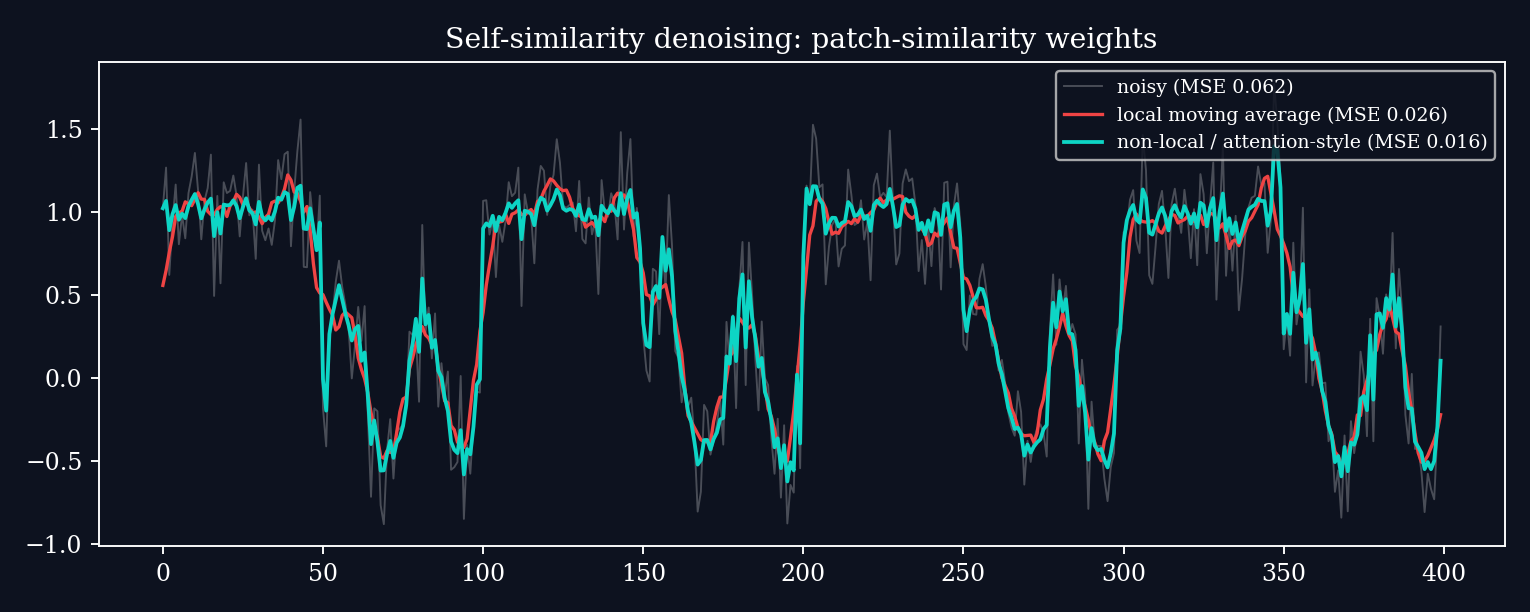
\includegraphics[width=0.95\textwidth]{images/l28_nonlocal_attention.png}
\caption{Toy 1-D demonstration: a piecewise signal with repeating structure is denoised either by a local moving average or by similarity-weighted (attention-style) averaging over all positions. Self-similarity lets distant, similar patches reinforce each other without blurring edges. (Parameters here were tuned by hand for illustration only.)}
\end{figure}

\textbf{Caveats.} BM3D has hand-designed transforms, hard thresholds and a fixed patch metric; attention weights are learned, use projected features $\mathbf{W}_Q,\mathbf{W}_K,\mathbf{W}_V$, run several heads and have no explicit threshold. The correspondence is conceptual (non-local self-similarity), not an identity of algorithms.

\noindent\rule{\textwidth}{0.5pt}

\section{8. POSITIONAL ENCODING IS A BANK OF PHASORS}

Self-attention is permutation-invariant, so positions must be injected. The original Transformer adds
\begin{equation}
PE(p,2i)=\sin(\omega_i p),\quad PE(p,2i+1)=\cos(\omega_i p),\qquad \omega_i=10000^{-2i/d}.
\end{equation}
Each pair $(\sin,\cos)$ is the real and imaginary part of a phasor $e^{j\omega_i p}$ rotating with position (``time'' is position $p$). The frequencies are \textbf{geometrically spaced} from $\omega_0=1$ rad/token down to $\approx 10^{-4}$ rad/token (wavelengths $2\pi$ up to $\approx 6\times10^4$ tokens) --- like a multi-resolution filter bank, or like binary digits of a counter where each bit flips at a different rate.

\subsection{8.1 Shift = rotation}
\begin{equation}
\begin{bmatrix}\sin\omega(p+k)\\ \cos\omega(p+k)\end{bmatrix}
=\underbrace{\begin{bmatrix}\cos\omega k&\sin\omega k\\-\sin\omega k&\cos\omega k\end{bmatrix}}_{\mathbf{R}(\omega k)}
\begin{bmatrix}\sin\omega p\\ \cos\omega p\end{bmatrix}.
\end{equation}
This is the DFT shift theorem $x[p-k]\leftrightarrow e^{-j\omega k}X$: a position offset $k$ is a \emph{linear map independent of $p$}, so the network can learn to attend by relative offset. Moreover
\begin{equation}
PE(p)^T PE(p+k)=\sum_i\cos(\omega_i k),
\end{equation}
which depends only on $k$ --- exactly the autocorrelation of the phasor bank.

\subsection{8.2 Rotary embeddings (RoPE)}
RoPE does not add phasors but \emph{rotates} the query and key by $\mathbf{R}(\omega_i p)$ in each 2-D subspace; then $\langle \mathbf{R}(\omega p)\mathbf{q},\mathbf{R}(\omega p')\mathbf{k}\rangle=\mathbf{q}^T\mathbf{R}(\omega(p'-p))\mathbf{k}$, so attention depends on relative position only.

\subsection{8.3 Worked Example 28.3}
Take $d=8$: $\omega_i=10000^{-2i/8}$ for $i=0,1,2,3$: $1,\;0.1,\;0.01,\;0.001$ rad/token (wavelengths $6.28,\;62.8,\;628,\;6283$ tokens). For $\omega=1$, $p=2$, $k=1$: $PE=[\sin2,\cos2]=[0.909,-0.416]$. Applying $\mathbf{R}(1)$ with $\cos1=0.540$, $\sin1=0.841$:
\[
\sin3=0.540(0.909)+0.841(-0.416)=0.491-0.350=0.141,\quad \cos3=-0.841(0.909)+0.540(-0.416)=-0.765-0.225=-0.990,
\]
which matches $\sin3=0.141$, $\cos3=-0.990$.

\begin{figure}[H]
\centering
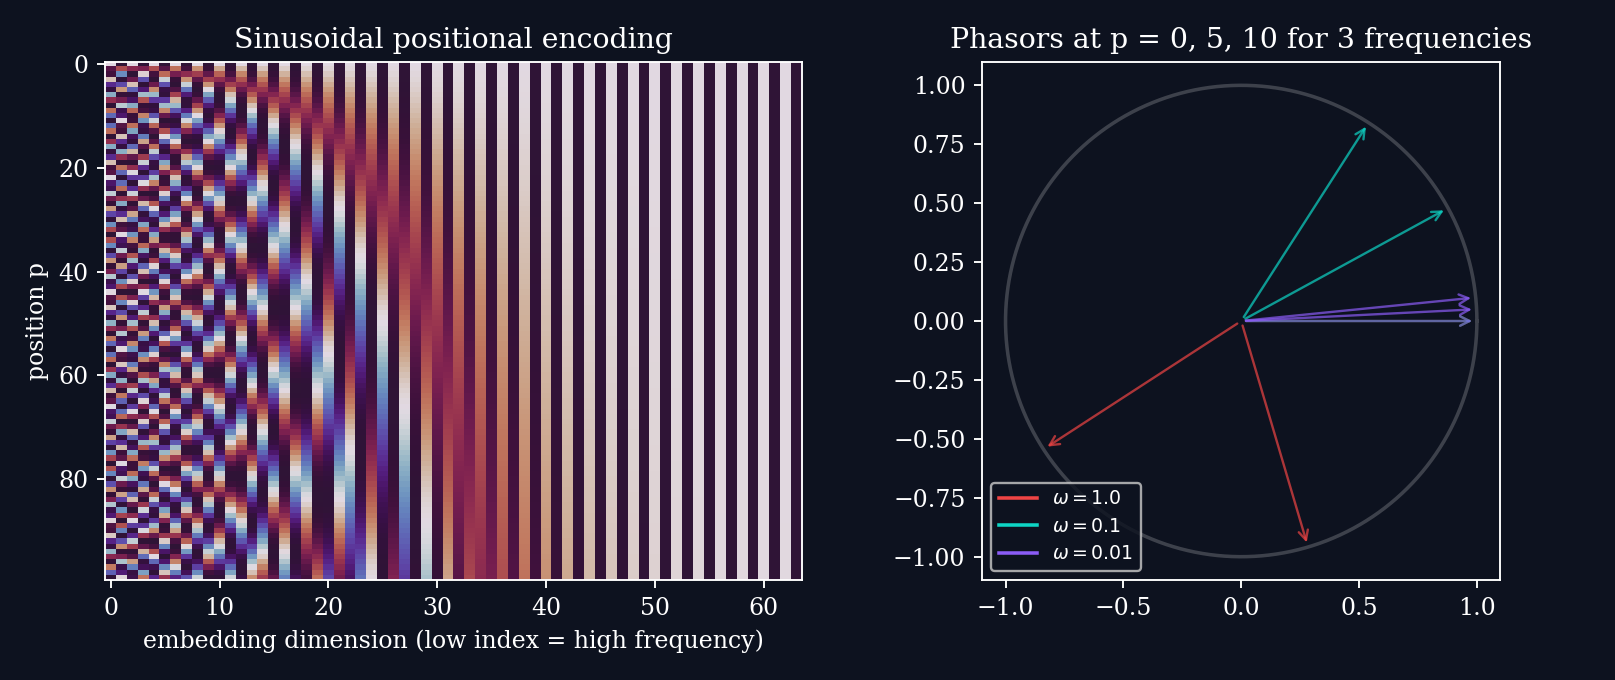
\includegraphics[width=0.95\textwidth]{images/l28_positional_phasors.png}
\caption{Left: sinusoidal positional encoding map ($d=64$): fast-oscillating columns at low index, slow at high index. Right: phasors at positions 0, 5, 10 for three frequencies --- high frequencies rotate quickly, low frequencies slowly.}
\end{figure}

\noindent\rule{\textwidth}{0.5pt}

\section{9. MORE SIMILARITIES}
\begin{table}[H]
\centering
\small
\begin{tabular}{p{4.2cm}p{4.4cm}p{6.0cm}}
\toprule
\textbf{DSP concept} & \textbf{ML concept} & \textbf{Comment} \\
\midrule
Matched filter / cross-correlation & Convolutional kernel as template detector; attention scores & Kernel responds maximally to the pattern it resembles; $\mathbf{q}^T\mathbf{k}$ is a correlation \\
Decimation + anti-alias filter & Strided conv/pooling; blur-pool & Strided CNNs alias; low-pass before downsampling improves shift-invariance \\
Filter banks, wavelets, multirate & Multi-scale CNNs, U-Net, feature pyramids & Analysis/synthesis structure with skip links \\
STFT / spectrogram & Input features for audio networks, ViT patches & Time-frequency tiling \\
Linear prediction / AR model & Autoregressive language models & Predict next sample (token) from the past; LPC is a linear ``language model'' \\
Kalman filter (state estimation) & Recurrent state estimation; SSMs & Predict--correct recursion with gain like a gate \\
Parallel/feed-forward path $y=x+F(x)$ & Residual connection & Direct path plus filtered path; improves gradient flow like a feed-forward comb \\
DC removal, AGC & Batch/Layer normalization & Remove mean, normalize power \\
Window functions, causal masks & Attention masks, causal attention & Restrict which samples contribute \\
Transform coding (DCT/JPEG) & Autoencoders, bottleneck codes & Compact representation, quantization = ``discrete latents'' \\
Compressed sensing, sparsity (L1) & Sparse coding, L1 regularization, pruning & Recovery from few measurements \\
Adaptive noise cancellation & Denoising networks, echo cancellers trained on reference & Reference correlated with noise, uncorrelated with signal \\
Lowpass smoothing, EMA & Momentum, EMA of weights, running stats & Section 4.3 \\
\bottomrule
\end{tabular}
\end{table}

\noindent\rule{\textwidth}{0.5pt}

\section{10. LIMITS OF THE ANALOGIES (EXAM TRAPS \& FACULTY INSIGHTS)}
\begin{itemize}
    \item \textbf{Linearity:} DSP filters (FIR/IIR) are linear and time-invariant; neural networks gain power from nonlinearities, so eigen/frequency analysis holds only for the linearized or linear versions.
    \item \textbf{Objectives differ:} LMS minimizes MSE with a convex quadratic bowl (unique minimum, guaranteed bound on $\mu$); deep networks have non-convex losses.
    \item \textbf{RNN poles:} eigenvalues of $\mathbf{W}_h$ are poles only for the \emph{linear} RNN; for $\tanh$, use the Jacobian along the trajectory.
    \item \textbf{BM3D vs.\ attention:} similar in spirit (non-local similarity-weighted aggregation), different in algorithmic detail.
    \item \textbf{Positional encoding:} the claim is not that Transformers perform a Fourier transform, but that sinusoidal PE is a set of phasors whose shift property gives relative-position information; learned or RoPE positional schemes exist.
    \item \textbf{Cross-correlation vs.\ convolution:} CNN ``convolution'' is cross-correlation (no kernel flip).
    \item \textbf{SVD vs.\ Fourier denoising:} Fourier works when the signal is \emph{band-limited}; SVD works when it is \emph{low rank}. A sum of sinusoids is both.
\end{itemize}

\noindent\rule{\textwidth}{0.5pt}

\section{11. QUICK REVISION CHEAT-SHEET}
\begin{table}[H]
\centering
\resizebox{\textwidth}{!}{
\begin{tabular}{lll}
\toprule
\textbf{Idea} & \textbf{Formula} & \textbf{ML name} \\
\midrule
LMS & $\mathbf{w}\leftarrow\mathbf{w}+\mu e\mathbf{x}$ & SGD / delta rule \\
Convergence along mode $i$ & $(1-\mu\lambda_i)^n$ & Condition number / learning-rate limit \\
One-pole IIR & $y[n]=a\,y[n-1]+(1-a)x[n]$ & EMA, momentum, forget gate \\
Linear RNN poles & $\mathrm{eig}(\mathbf{W}_h)$ & Vanishing/exploding gradients \\
LTI eigenfunction & $e^{j\omega n}\to H(e^{j\omega})e^{j\omega n}$ & Eigen-decomposition, PCA \\
Eckart--Young & $\min_{\mathrm{rank}\,k}\|\mathbf{A}-\mathbf{B}\|=\|\mathbf{A}-\mathbf{A}_k\|$ & Low-rank denoising, LoRA \\
NLM weights & $\mathrm{softmax}(-\|\mathbf{p}_i-\mathbf{p}_j\|^2/h^2)$ & Attention \\
Positional phasors & $e^{j\omega_i p},\ \omega_i=10000^{-2i/d}$ & Sinusoidal PE \\
Shift property & $PE(p+k)=\mathbf{R}(\omega k)PE(p)$ & Relative position, RoPE \\
\bottomrule
\end{tabular}
}
\end{table}

\end{document}
